\section*{Druckmessung}
Für die Druckmessung verwendet man Manometer (Druckmesser). Heutige Manometer funktionieren meistens
elektronisch. Hier wollen wir zwei Flüssigkeitsmanometer kennenlernen.
Das erste ist das offene U-Rohr-Manometer. Es besteht aus einem U-förmigen Rohr, das etwa halb mit einer Flüssigkeit
gefüllt ist. Herrscht auf beiden Seiten des U-Rohrs der gleiche Druck, so ist die Oberfläche auf der linken Seite
auf gleicher Höhe wie die Oberfläche auf der rechten Seite des U-Rohrs.
Wird auf einer Seite ein Überdruck ($P_{\textrm e}$) angelegt, so verschieben sich die Oberflächen gegeneinander.
Mit diesem Manometer kann man nur Druckdifferenzen messen.

\begin{minipage}{0.5\textwidth}
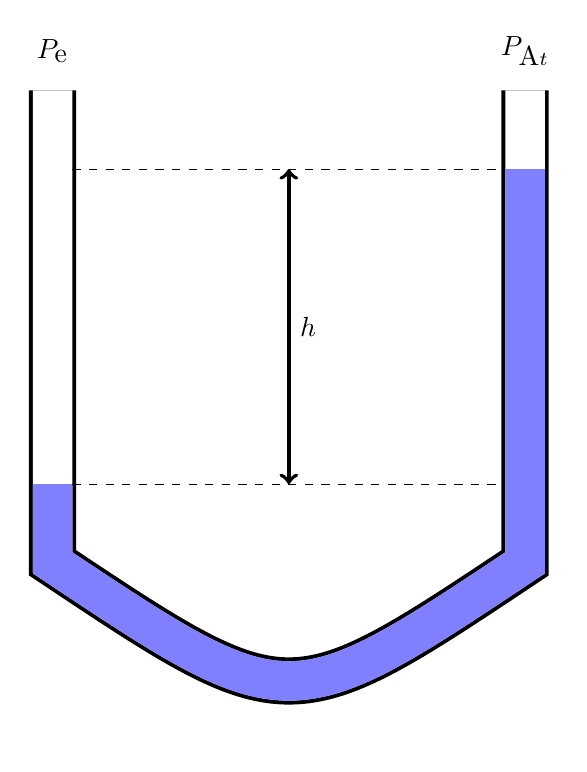
\begin{tikzpicture}[info text/.style={rounded corners, fill=red!20, inner sep=1ex}]
%\begin{tikzpicture}
\usetikzlibrary{calc,intersections,through,backgrounds}
\usetikzlibrary{decorations.pathmorphing}
%\draw[step=0.5cm,lightgray] (-0.5,-3.0) grid (6.5,5.0);

\draw [double distance=0.5cm, line width=0.05cm] (0,5)--(0,-1)..controls (3,-3) .. (6,-1)--(6,5);
\draw [line width=0.5cm,color=blue!50] (0,0)--(0,-1)..controls (3,-3) .. (6,-1)--(6,4);

\draw [dashed] (0.25,0)--(5.75,0);
\draw [dashed] (0.25,4)--(5.75,4);

%beschriftung der Höhe
\draw [<->, line width=0.05cm] (3,0)--(3,4);
\node at (3,2) [line width=0.05cm, right] {$h$};

%beschriftung Druck
\node at (6,5.5) {$P_{\textrm At}$};
\node at (0,5.5) {$P_{\textrm e}$};

\end{tikzpicture}
\end{minipage}
\begin{minipage}{0.5\textwidth}
Mit dem Höhenunterschied zwischen den beiden Oberflächen kann der Überdruck bestimmt werden. Es gilt


\begin{cbox}
	\begin{eqnarray*}
		P_{\textrm e}= \rho\cdot g\cdot h.
	\end{eqnarray*}
\end{cbox}

Dabei ist $\rho$ die Dichte der Flüssigkeit im inneren des U-Rohrs, $g$ die Fallbeschleunigung und $h$ der Höhenunterschied
zwischen beiden Oberflächen.
\end{minipage}


Heute sind diese Manometer nicht mehr sehr verbreitet.
Historisch wurde das offene Quecksilber Manometer zur Messung des Blutdrucks verwendet.
Die Einheit des Blutdrucks ist bis heute mmHg, also der Höhenunterschied von Quecksilber (Hg)
in einem offenen U-Rohr-Manometer.

\begin{aufgabe}
	\begin{itemize}
		\item[a)] Wie hoch ist der Druck von \SI{120}{mmHg} in der für den Druck üblichen Einheit Pascal?
		\item[b)] Welchem Höhenunterschied entspricht dass, wenn stattdessen Wasser im Manometer verwendet wird?
	\end{itemize}

	\begin{loesung}
	\begin{itemize}
		\item[a)]
		\begin{eqnarray*}
			P=\rho_{\textrm Hg}\cdot g\cdot h = \SI{13546}{kg/m^3}\cdot \SI{10}{N/kg}\cdot\SI{0.12}{m}=\SI{1.6255e+4}{Pa}
		\end{eqnarray*}
	\item[b)]
		\begin{eqnarray*}
			P=\rho\cdot g\cdot h \to h= \frac{P}{\rho\cdot g}=\frac{\SI{1.6255E4}{Pa}}{\SI{1000}{kg/m^3}\cdot \SI{10}{N/kg}}=\SI{1.63}{m}
		\end{eqnarray*}

\end{itemize}
	\end{loesung}
\end{aufgabe}

Eine Variation des offenen Manometers ist das geschlossene Manometer. Mit diesem werden keine Druckdifferenzen gemessen,
wie beim offenen Manometer sondern absolute Drücke.

\begin{minipage}{0.5\textwidth}
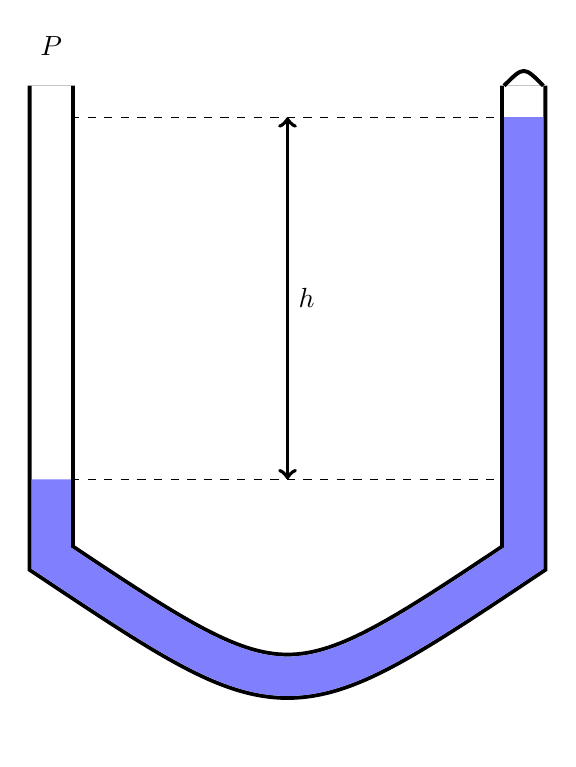
\begin{tikzpicture}[info text/.style={rounded corners, fill=red!20, inner sep=1ex}]
%\begin{tikzpicture}
\usetikzlibrary{calc,intersections,through,backgrounds}
\usetikzlibrary{decorations.pathmorphing}
%\draw[step=0.5cm,lightgray] (-0.5,-3.0) grid (6.5,5.0);

\draw [double distance=0.5cm,line width=0.05cm] (0,5)--(0,-1)..controls (3,-3) .. (6,-1)--(6,5);
\draw [line width=0.05cm] (5.75,5)..controls (6,5.25)..(6.25,5);

\draw [line width=0.5cm,color=blue!50] (0,0)--(0,-1)..controls (3,-3) .. (6,-1)--(6,4.6);

\draw [dashed] (0.25,0)--(5.75,0);
\draw [dashed] (0.25,4.6)--(5.75,4.6);

%beschriftung der Höhe
\draw [<->, line width=0.05cm] (3,0)--(3,4.6);
\node at (3,2.3) [line width=0.05cm, right] {$h$};

%beschriftung Druck
%\node at (6,5.5) {$P_{\textrm At}$};
\node at (0,5.5) {$P$};

\end{tikzpicture}
\end{minipage}
\begin{minipage}{0.5\textwidth}

	Mit dem Höhenunterschied zwischen den beiden Oberflächen kann der Druck bestimmt werden. Es gilt


\begin{cbox}
	\begin{eqnarray*}
		P= \rho\cdot g\cdot h.
	\end{eqnarray*}
\end{cbox}

Dabei ist $\rho$ die Dichte der Flüssigkeit im inneren des U-Rohrs, $g$ die Fallbeschleunigung und $h$ der Höhenunterschied
zwischen beiden Oberflächen.
In der geschlossenen Röhre bildet sich oben ein Vakuum. Im Vakuum ist der Druck Null. Deshalb kann
in diesem Manometer der Druck gemessen werden.
\end{minipage}
Historisch wird dieser Manometertyp zur Messung des Luftdrucks verwendet.
Der Normaldruck von \SI{1013}{hPa} entspricht einer Quecksilbersäule von \SI{76}{cm}.

\begin{aufgabe}
	In einem Experiment sehen Sie ein geschlossenes Quecksilbermanometer unter einer Glasglocke.
	Mit der Vakuumpumpe wird die Luft aus der Glasglocke gepumpt.
	Lesen Sie den Höhenunterschied zwischen den zwei Flüssigkeitsoberflächen ab und bestimmen Sie den Druck unter der Glasglocke.
\end{aufgabe}
